\begin{pastexam}[label={px:ntu-108-comm-dsab-23}]{臺大電信所 108 學年度（B）第 23 題}
（單選；每題 2.5 分，答錯不倒扣）

In a red-black tree, suppose there is a path with 3 red nodes, then there are at least how many
black nodes in the tree?

A.~0 \qquad B.~4 \qquad C.~7 \qquad D.~8 \qquad E.~11
\end{pastexam}

\begin{pastsoln}
答案是 E。

「path」解讀成從根往下到葉的一條路徑（紅黑樹的性質都是針對這種路徑說的）。 下面的「黑高」數的是
一個節點往下到 NIL 的路徑上，黑色內部節點的個數（自己是黑的也算），NIL 不算。

\textbf{一個引理}：黑高 $h$ 的子樹至少有 $2^h - 1$ 個黑色節點。 對 $h$ 歸納：$h = 0$ 時是 $0$ 個。
根是黑的，兩個子節點的黑高都是 $h - 1$，至少 $1 + 2(2^{h-1} - 1) = 2^h - 1$ 個；根是紅的，兩個子節點
都是黑高 $h$ 的黑節點（或 $h = 0$ 時的 NIL），至少 $2(2^h - 1) \ge 2^h - 1$ 個。

\textbf{下界}：根是黑的、紅節點不相鄰，所以一條有 $3$ 個紅節點的路徑上至少有 $3$ 個黑節點，樹的黑高
$h \ge 3$。 如果 $h \ge 4$，由引理已經至少 $15$ 個黑節點。 如果 $h = 3$，這條路徑上剛好 $3$ 黑
$3$ 紅，只能是 黑$_1$、紅$_1$、黑$_2$、紅$_2$、黑$_3$、紅$_3$（紅$_3$ 底下是 NIL）。 路徑上每個節點
的「另一個子節點」都是一棵獨立的子樹，黑高由位置決定：
\begin{center}
\begin{tabular}{lcc}
\toprule
路徑上的節點 & 另一個子樹的黑高 & 至少幾個黑節點 \\
\midrule
黑$_1$（根） & 2 & 3 \\
紅$_1$ & 2（必須是黑節點） & 3 \\
黑$_2$ & 1 & 1 \\
紅$_2$ & 1（必須是黑節點） & 1 \\
黑$_3$ & 0（NIL） & 0 \\
\bottomrule
\end{tabular}
\end{center}
加上路徑上的 $3$ 個黑節點，總共至少 $3 + 3 + 3 + 1 + 1 = 11$ 個。

\textbf{做得到}：照上表每個子樹都取最小的（黑高 $2$ 取一個黑節點帶兩個黑葉，黑高 $1$ 取一個黑葉），
就是下圖，黑節點（實心）剛好 $11$ 個，每條到 NIL 的路徑都經過 $3$ 個黑節點，紅節點（R）都不相鄰：
\begin{center}
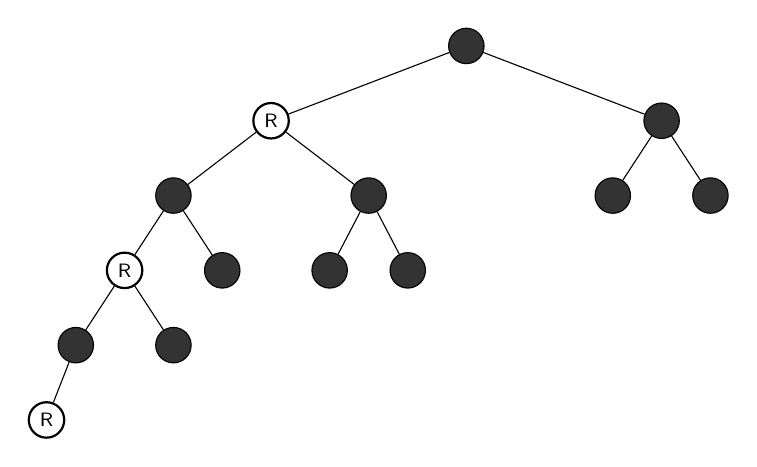
\begin{tikzpicture}[x=0.62cm,y=0.95cm,
  b/.style={circle,draw,fill=black!80,inner sep=0pt,minimum size=4.5mm},
  r/.style={circle,draw,thick,fill=white,inner sep=0pt,minimum size=4.5mm,font=\scriptsize\sffamily}]
\node[b] (b1) at (8,0) {};
\node[r] (r1) at (4,-1) {R};
\node[b] (x) at (12,-1) {};
\node[b] (x1) at (11,-2) {}; \node[b] (x2) at (13,-2) {};
\node[b] (b2) at (2,-2) {};
\node[b] (y) at (6,-2) {};
\node[b] (y1) at (5.2,-3) {}; \node[b] (y2) at (6.8,-3) {};
\node[r] (r2) at (1,-3) {R};
\node[b] (z) at (3,-3) {};
\node[b] (b3) at (0,-4) {}; \node[b] (b3p) at (2,-4) {};
\node[r] (r3) at (-0.6,-5) {R};
\draw (b1)--(r1) (b1)--(x) (x)--(x1) (x)--(x2) (r1)--(b2) (r1)--(y) (y)--(y1) (y)--(y2)
      (b2)--(r2) (b2)--(z) (r2)--(b3) (r2)--(b3p) (b3)--(r3);
\end{tikzpicture}
\end{center}
所以答案是 $11$。 C 的 $7 = 2^3 - 1$ 只用了「黑高至少 $3$」，忘了每個紅節點底下要接兩棵同黑高的
子樹；A、B、D 也都比 $11$ 小。
\end{pastsoln}
